paragraph{Examples with Predication: }

This next example illustrates a switch of a DEE path to become
the new main-line path.
Consider the following code sequence.

\begin{verbatim}

00	r2 <- r0 op r1
10	b_op r2, 030
20	r3 <- r0 op r1
30	r4 <- r0 op r1

\end{verbatim}

The time ordered execution sequence for this example is shown in
Figure~\ref{pex3}.

\begin{figure}
\centering
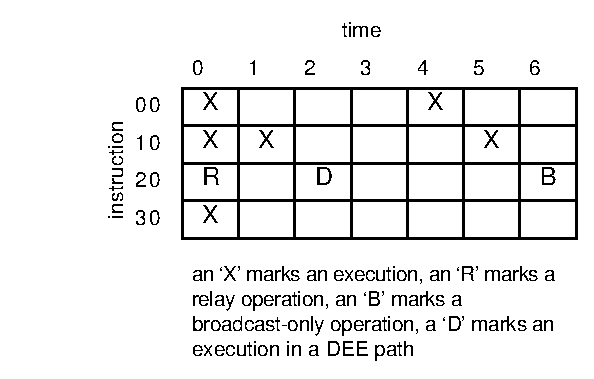
\epsfig{file=pex3.eps,width=2.50in}
\caption{{\em Timing of the code example, predication scenario 3.}
This example illustrates a switch of a DEE path to
become the new main-line path.
Execution of an instruction at a given time is
again indicated by an `X', a relay operation is indicated by an 'R',
and a broadcast-only operation is indicated by a 'B'.}
\label{pex3}
\end{figure}

It is assumed that all instructions are loaded and that
the branch at 10 is initially predicted as taken.
It is also assumed that all of the instructions are
executed immediately in main-line active stations.
Note that the execution of instruction 20 is really only
just a relay operation because it is within the domain of the branch 
in instruction 10 and the initial prediction is taken.
Because instruction 10 is data dependent on instruction 00, it
sees the newly broadcasted value
for register
{\tt r2}
from instruction 00 and becomes enabled to execute again.
It executes again in cycle 1.
This current state of execution, with regard to the instructions
shown, may persist for some time until the committed state of
the machine catches up with the current instructions.

It is now assumed that a DEE path was created, some time
after the initial executions already mentioned, and that
instruction 20 gets to execute in the DEE path.  Since
the DEE path branch output predicate is always opposite of
that of the same branch in the main-line active stations,
instruction 20 executes creating a new value for
register
{\tt r3}
rather than relaying an old value as was done with this
same instruction in the main-line path.
This newly created value for register
{\tt r3}
is broadcast and may be snarfed by following both DEE path
active stations as well as following main-line path stations.
In this example, we have not shown any future instructions
dependent on the output of instruction 20 but there could be
some instructions executing in the instruction stream after instruction 30
as shown.

Finally, at some time later again, instruction 00
re-executes, creating what will become the resolved committed
state for register
{\tt r2}.
This enabled the re-execution of instruction 10, the branch.
When the branch executes, it also finally resolves.
We will assume that the branch resolves to the no-taken
state.  This is opposite to its previous prediction, indicating
a previous misprediction, and this will cause a switch of the
DEE path to become the new main-line path.
The effect of the DEE path switch to the main-line path
causes all predicated instructions following the branch
to re-broadcast their output values.  This is seen
happening with the broadcast-only operation of
instruction 20 in cycle 6.

Although, not shown in this example, instructions in the main-line
beyond the end of the DEE path (that was switched to main-line),
will also see the effects of the branch predicate change
if they were predicated at all (either directly or indirectly)
on the output resolution of the branch of instruction 10.

